\section{Freifunk: die Idee}
\subsection{Über Freifunk}

\begin{frame}
\frametitle{Was ist Freifunk überhaupt?}
	\begin{itemize}
		\item \href:{https://vimeo.com/64814620}{Video: Freifunk verbindet!}
		\item Aufbau eines vermaschten Netzwerkes $\rightarrow$ Meshnetz
		\item Demokratisierung einer Infrastruktur
		\item Zur Verfügung stellen freier Kommunikation für alle Personen $\leftrightarrow$ Offenes WLAN
		\item Netzneutralität
		\item Unabhängige \textbf{unkommerzielle Infrastruktur} in Bürgerhand
		\item Kostenlose, benutzerfreundliche \textbf{Hotspot-Gemeinschaft}
	\end{itemize}
\end{frame}

\begin{frame}
\frametitle{Wer macht Freifunk?}
	\begin{itemize}
		\item \textbf{Hierachiefreie}, \textbf{offene}, überregionale Gemeinschaft, die diese Grundsätze verfolgen will
		\item Personen, die \textbf{Router} aufstellen, \textbf{Firmware} schreiben oder \textbf{Server} bereitstellen
		\item Beginnt schon damit, dass eine Person einen Router für andere Menschen zur Verfügung stellt
		\item Unabhängige \textbf{unkommerzielle Infrastruktur} in Bürgerhand
		\item Dezentral weitflächig über Deutschland verteilt
	\end{itemize}
\end{frame}

\subsection{Wie funktioniert Freifunk?}

\begin{frame}
\frametitle{Wie funktioniert Freifunk?}
	\begin{itemize}
		\item WLAN-Mesh-Technologie “\textbf{Funk-Maschennetz}”
		\item Diese Technik eignet sich besonders gut um geografische und soziale Lücken zu schließen.
	\end{itemize}
	\begin{columns}[c]   
		\begin{column}[T]{0.4\textwidth}     
			\begin{itemize}
				\item \textbf{VPN vernetzt} „Inseln” und Städte
				\item Billig, Robust und ausfallsicher
				\item Für Alle immer frei und \textbf{unzensiert}
			\end{itemize}
		\end{column} 
		\begin{column}[T]{0.5\textwidth}     
			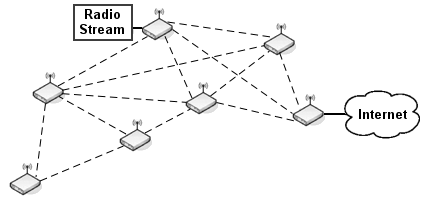
\includegraphics[width=\textwidth]{images/mesh_uebersicht.png}   
		\end{column}
	\end{columns} 
\end{frame}


\begin{frame}
\frametitle{Wohin geht welcher Traffic?}
	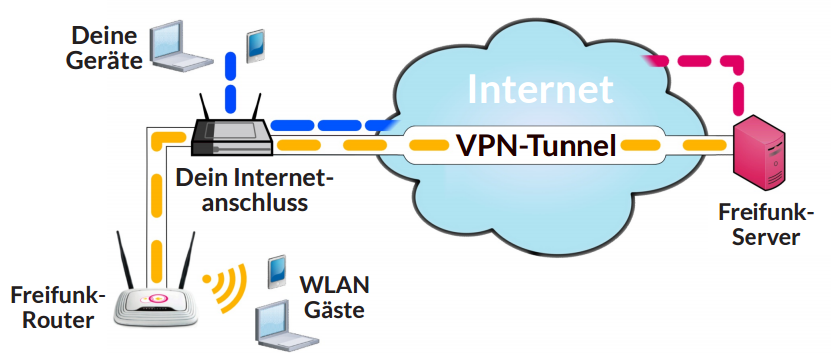
\includegraphics[scale=0.4]{images/personal_setup.png}
\end{frame}



\begin{frame}
\frametitle{}
	\begin{itemize}
		\item 
	\end{itemize}
\end{frame}
